\documentclass[10pt]{beamer}
\usetheme{Madrid}
\usecolortheme{orchid}
\usepackage[utf8]{inputenc}
\PassOptionsToPackage{hyphens}{url}
\usepackage{hyperref}
\usepackage{graphicx}
\usepackage{booktabs}
\usepackage{array}
\usepackage{xcolor}
\hypersetup{colorlinks=true, urlcolor=blue, linkcolor=black, breaklinks=true}
\urlstyle{same}

\title[Civic Monitor — Daily Update]{Civic Services Surveillance \& Monitoring}
\subtitle{Daily Progress Report — India-Specific Dataset Expansion}
\author{}
\institute{}
\date{31 August 2026}

\begin{document}

% ---------------------------------------------------------------
\begin{frame}
  \titlepage
\end{frame}

% ---------------------------------------------------------------
\begin{frame}{Agenda}
  \tableofcontents
\end{frame}

\section{Goal for Today}
% ---------------------------------------------------------------
\begin{frame}{Goal for Today}
  \textbf{Objective:} find and import \emph{genuinely India-specific} training data for
  each of the 7 civic-issue classes, organize it classwise, and separate a final
  curated "keep" set from the still-being-reviewed pool.
  \vspace{0.5em}
  \begin{itemize}
    \item Prior sessions' data was mostly non-Indian imagery (Roboflow/Kaggle sources
      picked for class relevance, not geography).
    \item Only 2--3 of $\sim$13 existing sources were confirmed India-specific before today.
    \item Today: deep per-class research, strict visual verification of every candidate
      before use, classwise organization, and dashboard-based curation.
  \end{itemize}
\end{frame}

\section{Method: Verify, Don't Trust the Title}
% ---------------------------------------------------------------
\begin{frame}{Method: Verify, Don't Trust the Title}
  Every candidate dataset was \textbf{downloaded and visually sample-checked} before
  being trusted — titles and workspace branding were repeatedly misleading:
  \begin{itemize}
    \item \texttt{IIT-Madras/pothole-detection} $\to$ sample image was an African township storefront.
    \item \texttt{Smart-India-Hackathon/final-garbage} $\to$ sample was a Bigstock stock photo of
      \emph{Indonesian} grocery brands.
    \item \texttt{sakshi-kumari/cow-indian} $\to$ same dataset already rejected in an earlier
      session (tight face/nose crops, not road scenes) — re-surfaced by search without
      history cross-check.
    \item \texttt{pib-e46kr/indian-bovine} $\to$ genuine Indian breed dataset, but close-up
      farm/breed-showcase photography, not road scenes.
  \end{itemize}
  \textbf{Lesson:} accept nothing on title/workspace name alone — open real sample images first.
\end{frame}

\section{Data Collected Today}
% ---------------------------------------------------------------
\begin{frame}{Data Collected Today — Summary}
  \begin{center}
  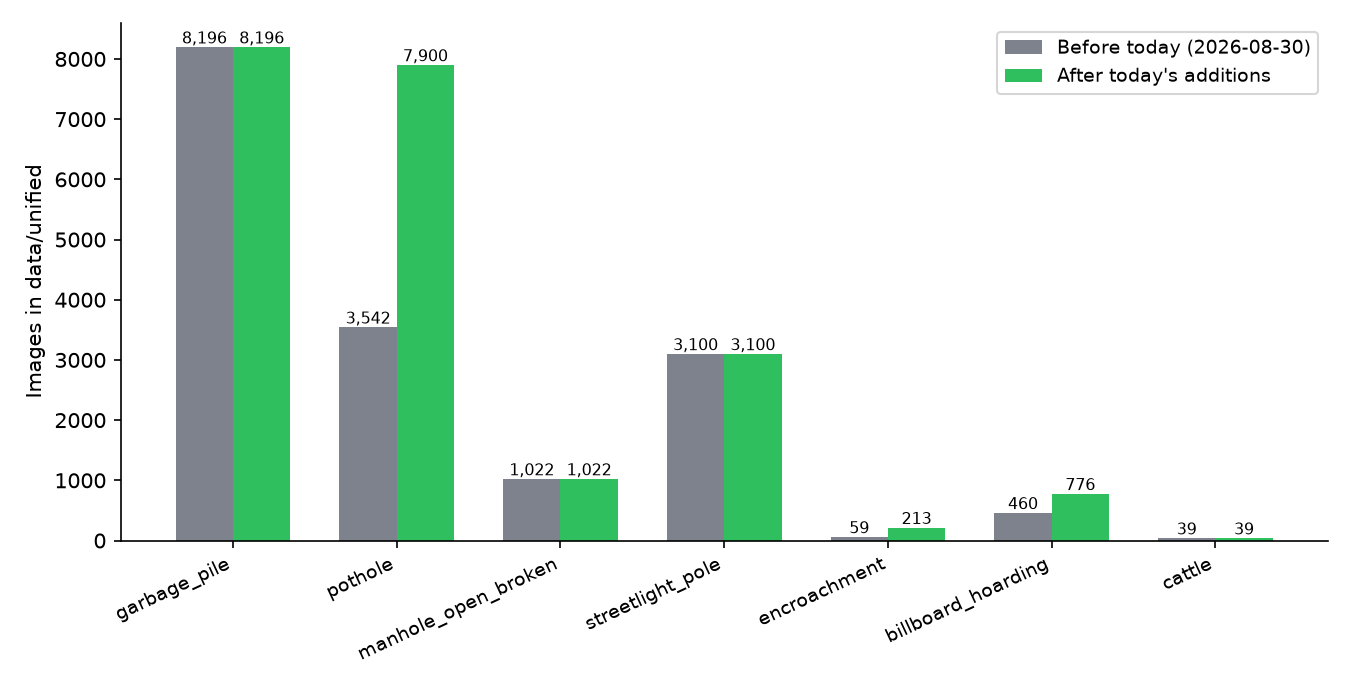
\includegraphics[width=0.95\textwidth]{images/class_counts_chart.png}
  \end{center}
\end{frame}

\begin{frame}{Data Collected — Source Detail}
  \tiny
  \begin{tabular}{p{2.0cm}p{2.9cm}p{0.9cm}p{3.4cm}}
    \toprule
    \textbf{Class} & \textbf{Source} & \textbf{Added} & \textbf{Evidence of India origin} \\
    \midrule
    Pothole & \texttt{indian-road-potholes} (Roboflow) & 4,306 & Scooters, whitewashed compound walls, Indian apartment architecture \\
    Pothole & \texttt{bharat-pothole}, India-tagged subset & 52 & Auto-rickshaw, Indian truck design, roadside signage \\
    Billboard & \texttt{advision/ooh-detection} & 316 & 360° footage on CG Road, Ahmedabad; AMTS (Ahmedabad transport) taxonomy \\
    Encroachment & \texttt{vendor/footpath-guide-2} & 154 & Palm-lined streets, Indian utility poles, vendor cart on footpath \\
    Streetlight & Chennai Working/NotWorking set & 718* & Academic dataset (arXiv:2407.01117), captured across Chennai \\
    \bottomrule
  \end{tabular}
  \vspace{0.5em}
  \footnotesize *Classification-format (whole-image label, no boxes) — see "Current Work in Progress".
\end{frame}

\section{Sample Images}
% ---------------------------------------------------------------
\begin{frame}{Sample: Pothole (India-confirmed)}
  \centering
  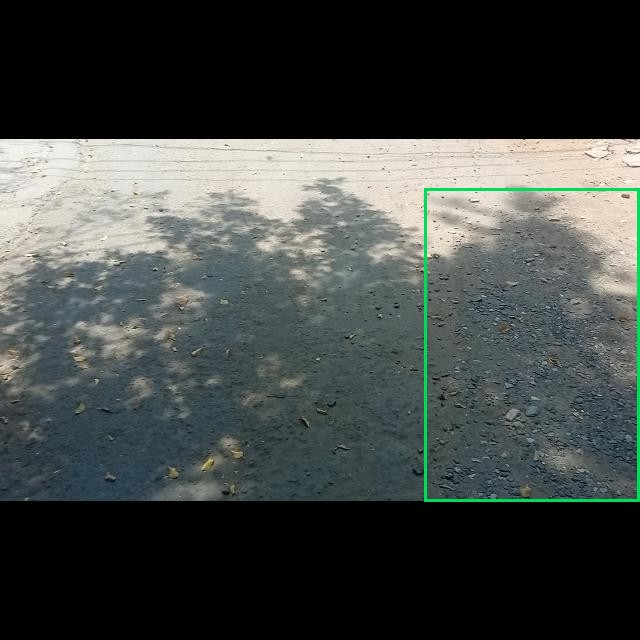
\includegraphics[height=0.42\textheight]{images/pothole_india_1.jpg}\hspace{0.5em}
  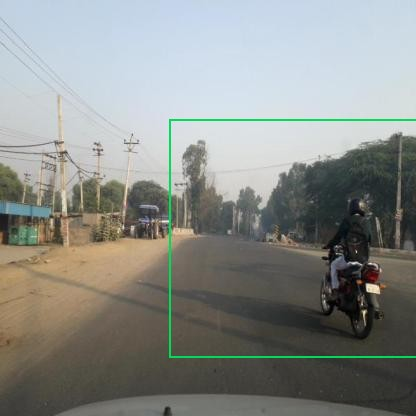
\includegraphics[height=0.42\textheight]{images/pothole_india_2.jpg}\\
  \footnotesize Left: indian-road-potholes. Right: bharat-pothole (India-tagged subset).
\end{frame}

\begin{frame}{Sample: Billboard/Hoarding \& Encroachment}
  \centering
  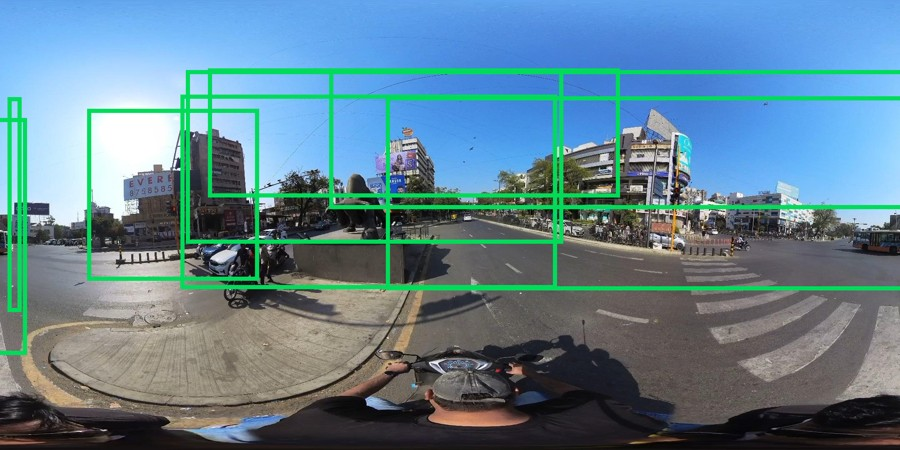
\includegraphics[height=0.42\textheight]{images/billboard_india_1.jpg}\hspace{0.5em}
  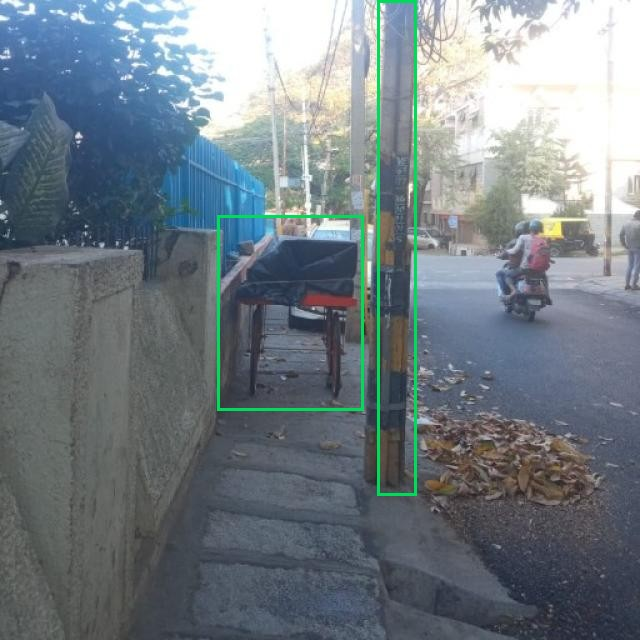
\includegraphics[height=0.42\textheight]{images/encroachment_india_1.jpg}\\
  \footnotesize Left: CG Road, Ahmedabad hoardings. Right: vendor cart obstructing footpath.
\end{frame}

\begin{frame}{Sample: Streetlight — Working vs Not Working}
  \centering
  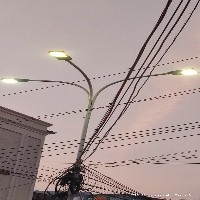
\includegraphics[height=0.42\textheight]{images/streetlight_working.jpg}\hspace{0.5em}
  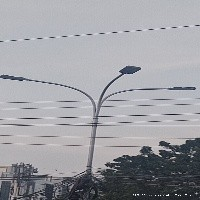
\includegraphics[height=0.42\textheight]{images/streetlight_notworking.jpg}\\
  \footnotesize Left: working. Right: non-functional. Chennai, India — 444 / 274 images.
\end{frame}

\section{Curated Training Set}
% ---------------------------------------------------------------
\begin{frame}{Curated "Keep" Training Set Split Out}
  \begin{itemize}
    \item Reviewed images in the dashboard (\texttt{review\_tool.py}) marked \textbf{Keep}
      were moved (not copied) out of \texttt{data/unified/} into a new classwise folder:
      \texttt{data/training\_data/<class>/\{train,val\}/\{images,labels\}}
    \item \texttt{data/unified/} now holds only the still-unreviewed / discarded pool —
      the dashboard's counts dropped accordingly.
    \item New read-only viewer built for the curated set:
      \texttt{training\_data\_dashboard.py} — \url{http://127.0.0.1:5070}
  \end{itemize}
  \vspace{0.5em}
  \small
  \begin{tabular}{lr}
    \toprule
    \textbf{Class} & \textbf{Curated (kept) images} \\
    \midrule
    manhole\_open\_broken & 267 \\
    garbage\_pile & 128 \\
    pothole & 125 \\
    streetlight\_pole & 101 \\
    billboard\_hoarding & 98 \\
    encroachment & 59 \\
    cattle & 39 \\
    \midrule
    \textbf{Total} & \textbf{817} \\
    \bottomrule
  \end{tabular}
\end{frame}

\section{Current Work in Progress / Blocker}
% ---------------------------------------------------------------
\begin{frame}{Current Work in Progress}
  \textbf{Streetlight functional/non-functional annotation} (separate terminal session,
  in progress right now):
  \begin{itemize}
    \item The 718 Chennai streetlight photos are \textbf{classification-format} (whole-image
      Working/NotWorking label) — not usable directly by the box-based YOLO merge pipeline.
    \item First attempt: automatic zero-shot labeling (YOLO-World) — \textbf{rejected}, too
      inaccurate ($\sim$40\% miss rate on real poles).
    \item Now building manual annotation instead: a dedicated tool
      (\texttt{streetlight\_annotate.py}, port 5052) to draw boxes by hand.
    \item Status as of this report: tool is built and tested end-to-end, but
      \textbf{annotation has not started yet} — 0 / 443 Working, 0 / 273 NotWorking done.
  \end{itemize}
  \textcolor{red}{\textbf{This is the open item blocking streetlight\_pole from benefiting
  from today's new data.}}
\end{frame}

\section{Classes Still Missing Good India Data}
% ---------------------------------------------------------------
\begin{frame}{Classes Still Missing Good India Data}
  Despite a real search effort (Roboflow API, GitHub, Kaggle, academic sources), no
  credible India-specific data was found for:
  \begin{itemize}
    \item \textbf{Garbage on road} — the one "Smart India Hackathon" lead was actually an
      Indonesian stock photo; Kaggle lead unverifiable (no Kaggle credentials in this
      environment). \textbf{Weakest class along with cattle.}
    \item \textbf{Manhole (open/broken)} — one source has a "manhole" class, but doesn't
      distinguish open/broken from closed/intact — same contamination risk already
      flagged for the existing dataset, so not merged.
    \item \textbf{Cattle on road} — two more candidates checked, both close-up farm/breed
      photography, not road scenes. Existing 39-image India source remains the best
      (already strong, AP50 0.986 in the last trained model).
  \end{itemize}
  \vspace{0.3em}
  \small These three classes need either a Kaggle account + real verification, or
  self-collection — not more automated dataset search.
\end{frame}

\section{Next Steps}
% ---------------------------------------------------------------
\begin{frame}{Next Steps}
  \begin{enumerate}
    \item Finish manual streetlight Working/NotWorking annotation (other terminal, in progress).
    \item Decide streetlight integration path: separate lit/unlit classifier vs.
      hand-boxed detection data.
    \item Continue per-class review in \texttt{review\_tool.py} for pothole and
      manhole\_open\_broken (largely untouched pools).
    \item Set up Kaggle credentials to verify the one remaining garbage-dataset lead.
    \item Retrain YOLO11n once the curated \texttt{data/training\_data/} set is more complete
      — not yet retrained on any of today's changes.
  \end{enumerate}
\end{frame}

\end{document}
